\chapter{Validazione e Test del Sistema}

Il presente capitolo espone i risultati delle procedure di validazione effettuate sull'architettura sviluppata, articolandosi in due ambiti di analisi principali: i test prestazionali e i test di sicurezza.

\section{Test Prestazionali e di Carico (Postman)}

In questa sezione vengono presentati i risultati dei test di carico e affidabilità condotti sulle API dell'applicazione sviluppata. L'obiettivo dell'analisi è verificare la resilienza, i tempi di risposta e la stabilità del backend simulando diversi scenari di accesso concorrente, al fine di individuare potenziali colli di bottiglia o vulnerabilità legate alla disponibilità del servizio (es. mitigazione di attacchi di tipo \textit{Denial of Service} elementari o problemi di gestione delle risorse).

\subsection{Ambiente di Test e Premessa Metodologica}
I test sono stati eseguiti all'interno di un ambiente controllato in locale (\textit{localhost}). Per garantire la replicabilità dei risultati, si riportano di seguito le specifiche hardware delle macchine ospitanti su cui sono stati eseguiti sia l'applicazione sia l'istanza dello strumento di testing:

\begin{itemize}
    \item \textbf{PC portatile}: \textbf{CPU:} AMD Ryzen 7 4000, \textbf{Memoria RAM:} 16 GB DDR4, \textbf{GPU:} Non dedicata 
    \item \textbf{PC fisso}: \textbf{CPU:} AMD Ryzen 9 9900X (12c, 24t), \textbf{Memoria RAM:} 32 GB DDR5, \textbf{GPU:} NVIDIA 5070Ti (16 GB VRAM) 
    \item \textbf{Strumento di Testing:} Postman
\end{itemize}

\textit{Nota di contesto:} L'assenza di una GPU dedicata sul PC portatile influisce sulle prestazioni metriche dell'applicazione, in quanto il carico di lavoro del modello di IA è interamente gravato sulla CPU e sulla memoria RAM.

\subsection{Analisi dei Risultati e Scenari di Carico}
I test effettuati hanno simulato diverse curve di carico misurate in \textit{Virtual Users} (VU). Di seguito vengono analizzati nel dettaglio i singoli scenari eseguiti.

\subsubsection{PC portatile}
\begin{table}[H] % <--- Forzato il posizionamento qui
\centering
\small
\caption{Metriche delle prestazioni registrate su Postman (PC portatile)}
\label{tab:test_postman_portatile}
\begin{tabular}{lccccc}
\toprule
\textbf{Scenario di Test} & \textbf{Profilo di Carico} & \textbf{Tempo Medio (Avg)} & \textbf{Tempo Max} & \textbf{Durata} \\
\midrule
Carico Costante & 5 VU costanti & $\sim$950 ms & 1.6 s & 3 min  \\
Rampa Lineare & Da 1 a 5 VU & $\sim$1.0 s (a regime) & -- & Var.\\
Picco Repentino & Spike 5 VU & -- & 1.0 s & Impuls. \\
Picco Repentino & Spike 10 VU & -- & 2.0 s & Impuls. \\
Rampa Incrementale & Da 1 a 10 VU & $\sim$1.5 s (a regime) & -- & Var. \\
\bottomrule
\end{tabular}
\end{table}

\subsubsection{PC fisso}
\begin{table}[H] % <--- Forzato il posizionamento qui
\centering
\small
\caption{Metriche delle prestazioni registrate su Postman (PC fisso)}
\label{tab:test_postman_fisso}
% Centra la tabella ignorando i margini del testo
\makebox[\textwidth][c]{
    \begin{tabular}{lcccc} % Corretto da lccccc a lcccc (5 colonne)
    \toprule
    \textbf{Scenario di Test} & \textbf{Profilo di Carico} & \textbf{Tempo Medio (Avg)} & \textbf{Tempo Max} & \textbf{Durata} \\
    \midrule
    Carico Costante & 5 VU costanti & $\sim$21 ms & 1 s & 2 min  \\
    Rampa Lineare & Da 1 a 5 VU & $\sim$17 ms a regime & -- & 2 min\\
    Carico Costante & 20 VU costanti & $\sim$32 ms & 1.6 s & 2 min  \\
    Rampa Lineare & Da 1 a 20 VU & $\sim$16 ms a regime & -- & Var.\\
    Picco Repentino & Spike 20 VU & -- & 4.0 s & Impuls. \\
    Rampa Lineare & Da 1 a 30 VU & $\sim$18 ms a regime & -- & Var.\\
    Rampa Lineare up\&down & 30 VU & 18 ms (40 ms a regime) & 1.65 s & -- \\
    Picco Repentino & Spike 30 VU & -- & 7.0 s & Impuls. \\
    Rampa Lineare up\&down & 100 VU & 268 ms (500 ms a regime) & 3 s & 2 min \\
    \bottomrule
    \end{tabular}
}
\end{table}


\begin{figure}[H] % <--- Forzato il posizionamento qui
    \centering
    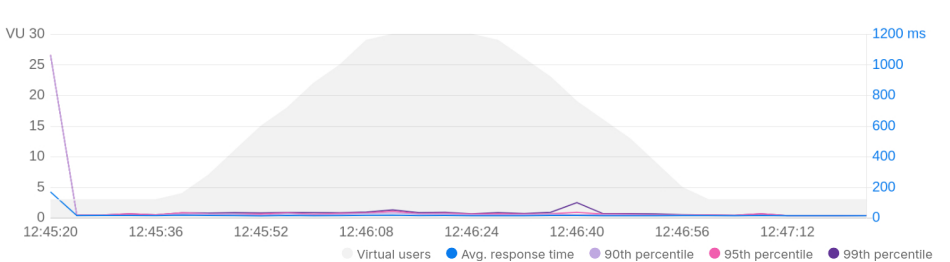
\includegraphics[width=1.0\textwidth]{immagini/peak30uv.png}
    \caption{Grafico Peak 30 VU}
    \label{fig:peak30uv}
\end{figure}

\begin{figure}[H] % <--- Forzato il posizionamento qui
    \centering
    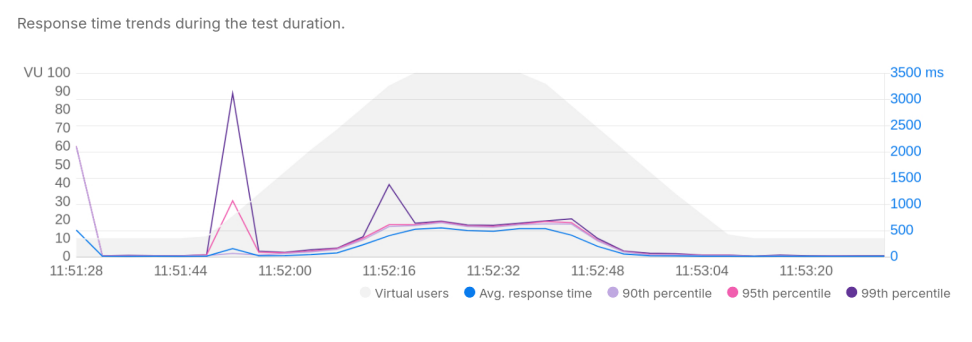
\includegraphics[width=1.0\textwidth]{immagini/peak100uv.png}
    \caption{Grafico Peak 100 VU}
    \label{fig:peak100uv}
\end{figure}

\subsubsection{Considerazioni Tecniche}

L'esecuzione dei test di carico a volumi di traffico reali ha permesso di delineare con maggiore precisione i limiti di scalabilità e la robustezza del backend sviluppato. L'analisi dei dati aggregati nelle tabelle \ref{tab:test_postman_portatile} e \ref{tab:test_postman_fisso} evidenzia i seguenti comportamenti del sistema:

\begin{itemize}
    \item \textbf{Efficienza in Condizioni Standard (Saturazione Bassa/Media):} Nello scenario a carico costante con 5 VU, il sistema risponde con un tempo medio estremamente ridotto ($\sim$21~ms). Questo valore, unito ai $\sim$32~ms registrati con 20 VU costanti, dimostra l'ottima efficienza della logica di routing e della gestione dei thread.
    
    \item \textbf{Scalabilità Lineare e Curve di Ramp-up:} I test di \textit{Ramp-up} lineare (fino a 5, 20 e 30 VU) mostrano un comportamento quasi ottimale, con tempi a regime stabili tra i $16\text{ ms}$ e i $18\text{ ms}$. Il server si dimostra capace di allocare dinamicamente le risorse necessarie man mano che nuove connessioni vengono stabilite, senza subire degradazioni prestazionali premature.
    
    \item \textbf{Analisi degli Scenari di Stress Avanzati (30 e 100 VU):} 
    Nel test \textit{Ramp-up up\&down} a 30 VU si nota un primo incremento del tempo a regime, che sale a $40\text{ ms}$. La vera e propria soglia di stress strutturale viene tuttavia raggiunta nello scenario a 100 VU (\textit{Ramp-up up\&down}): in questo caso il tempo medio globale si attesta a $268\text{ ms}$, ma subisce un raddoppio sensibile arrivando a $500\text{ ms}$ una volta raggiunto il pieno regime di carico.
    
    \item \textbf{Resistenza agli Spike:} 
    Lo \textit{Spike} a 20 VU mostra un tempo massimo di $4.0\text{ s}$, che sale linearmente a $7.0\text{ s}$ nello \textit{Spike} a 30 VU; anche nel \textit{Peak} a 100 VU in fase di salita è presente un tempo massimo di risposta di $3.0\text{ s}$. Questo incremento dei tempi di risposta massimi durante i picchi impulsivi evidenzia che il backend, pur non andando in \textit{crash}, soffre di un fenomeno temporaneo di \textit{saturazione delle risorse} quando riceve un numero anomalo di richieste improvvise, situazione che viene comunque assorbita superata la fase critica.
\end{itemize}

\section{Test di Sicurezza e Modello Zero Trust}

A completamento dell'analisi prestazionale, è stata condotta una batteria di test di sicurezza (eseguiti tramite una suite di test integrata nel cluster Docker) volti a verificare l'effettiva capacità dell'architettura Zero Trust di intercettare, valutare e neutralizzare pattern di attacco noti e comportamenti anomali. 

I test eseguiti hanno simulato sia attacchi frontali diretti contro il proxy esposto (Envoy), sia tentativi furtivi di movimento laterale diretti ai servizi interni, validando il funzionamento combinato del sistema di Intrusion Detection (Snort) e del decisore intelligente (AI Scorer).

\subsection{Scenari di Attacco Simulati}
La suite di test automatizzata ha replicato i seguenti scenari malevoli:
\begin{itemize}
    \item \textbf{SQL Injection (Mid-Level).} Simulazione di una query malevola all'endpoint delle API (\texttt{UNION SELECT * FROM users}), correttamente rilevata dalle regole Snort intermedie e bloccata (restituendo un errore 403 Forbidden).
    \item \textbf{Cross-Site Scripting (XSS).} Iniezione di uno script dannoso all'interno dei parametri di richiesta HTTP, parimenti neutralizzata dalla pipeline di sicurezza.
    \item \textbf{Utilizzo di Protocolli Obsoleti (Legacy TLS).} Invio di richieste di handshake SSLv3 forzate, le quali violano le policy di crittografia aggiornate e scatenano allarmi specifici a livello di rete.
    \item \textbf{Movimento Laterale Furtivo (Slowloris).} Per testare la resilienza alle minacce interne, il client ha bypassato volontariamente il proxy tentando una connessione diretta all'interfaccia dell'Orchestrator. Per eludere le rigide soglie volumetriche, l'attacco è stato condotto con la tecnica \textit{Slowloris}, trasmettendo un frammento di intestazione HTTP ogni due secondi, consumando le risorse senza destare allarmi di rete elementari.
\end{itemize}

\subsection{L'Intervento dell'AI Scorer}
Il banco di prova si è concluso con la verifica sul motore di intelligenza artificiale. A tale scopo è stata inviata una richiesta HTTP legittima (indirizzata a \texttt{/login}) e dotata di certificati crittografici validi, per innescare il flusso autorizzativo standard di Envoy verso l'Orchestrator.

Nonostante la richiesta risultasse formalmente valida, il sistema ha dimostrato un comportamento adattivo: l'AI Scorer ha analizzato la cronologia recente del client, che includeva i tentativi di attacco precedentemente simulati (tra cui il movimento laterale). Rilevando tali pattern anomali, il modello ha incrementato lo score di anomalia associato al client. Poiché il livello di rischio risultante ha superato le tolleranze consentite dalle policy in OPA, la richiesta è stata respinta preventivamente (HTTP 403 Forbidden).

Questi risultati confermano empiricamente che il sistema garantisce una validazione continua del comportamento, mitigando le minacce provenienti da entità compromesse prima che queste possano accedere alle risorse critiche dell'infrastruttura.